\documentclass[12pt]{article} % Default font size is 12pt, it can be changed here
\usepackage[utf8]{inputenc}
\usepackage{geometry} % Required to change the page size to A4
\geometry{a4paper} % Set the page size to be A4 as opposed to the default US Letter
\usepackage{listings}
\usepackage{parskip}
\usepackage{xcolor}
\usepackage{float}
\usepackage{graphicx} % Required for including pictures
\usepackage{hyperref}
\usepackage{float} % Allows putting an [H] in \begin{figure} to specify the exact location of the figure
\usepackage{cite}
\usepackage{fancyhdr}
\usepackage{lscape}

\linespread{1.2} % Line spacing

%\setlength{\parindent}{15pt}
%\setlength\parindent{0pt} % Uncomment to remove all indentation from paragraphs

\graphicspath{{../add/}} % Specifies the directory where pictures are stored

\pagestyle{fancy}
\lhead{Repositorio de árboles genealógicos en BD NoSQL}
\rhead{Daniel Albarral Nuñez}
\cfoot{\thepage}
\renewcommand{\headrulewidth}{0.4pt}
\renewcommand{\footrulewidth}{0.4pt}
\begin{document}

\begin{titlepage}

\newcommand{\HRule}{\rule{\linewidth}{0.5mm}} % Defines a new command for the horizontal lines, change thickness here

\center % Center everything on the page
 
%----------------------------------------------------------------------------------------
%	HEADING SECTIONS
%----------------------------------------------------------------------------------------

\textsc{\LARGE Universidad Politécnica de Cataluña}\\[1.5cm] % Name of your university/college
\textsc{\Large Facultad de Informática de Barcelona}\\[0.5cm] % Major heading such as course name
\textsc{\large Ingeniería de software}\\[0.5cm] % Minor heading such as course 

%----------------------------------------------------------------------------------------
%	TITLE SECTION
%----------------------------------------------------------------------------------------

\HRule \\[0.4cm]
{ \huge \bfseries Repositorio de árboles genealógicos en BD NoSQL}\\[0.4cm] % Title of your document
\HRule \\[1.5cm]
 
%----------------------------------------------------------------------------------------
%	AUTHOR SECTION
%----------------------------------------------------------------------------------------

\begin{minipage}{0.4\textwidth}
\begin{flushleft} \large
\emph{Author:}\\
Daniel \textsc{Albarral Nuñez} % Your name
\end{flushleft}
\end{minipage}
~
\begin{minipage}{0.4\textwidth}
\begin{flushright} \large
\emph{Supervisor:} \\
Enric \textsc{Mayol} % Supervisor's Name
\end{flushright}
\end{minipage}\\[4cm]

% If you don't want a supervisor, uncomment the two lines below and remove the section above
%\Large \emph{Author:}\\
%John \textsc{Smith}\\[3cm] % Your name

%----------------------------------------------------------------------------------------
%	DATE SECTION
%----------------------------------------------------------------------------------------

{\large Q1 - 2015-2016}\\[2cm] % Date, change the \today to a set date if you want to be precise

%----------------------------------------------------------------------------------------
%	LOGO SECTION
%----------------------------------------------------------------------------------------


\includegraphics[scale=0.7]{add/logo_upc.png}\\[1cm] % Include a department/university logo - this will require the graphicx package
 
%----------------------------------------------------------------------------------------

\vfill % Fill the rest of the page with whitespace

\end{titlepage}

%----------------------------------------------------------------------------------------
%   TABLE OF CONTENTS
%----------------------------------------------------------------------------------------

\tableofcontents % Include a table of contents

\newpage % Begins the essay on a new page instead of on the same page as the table of contents 

\section{Planificación temporal}
Como se ha explicado anteriormente para el desarrollo del proyecto se usara \textit{Scrum}, por ellos la planificación temporal estará estructurada para facilitar la consecución de esta metodología. El final del proyecto se ha establecido el 30 de junio de 2016.

\subsection{Gantt}
El gantt adjuntado a continuación tiene varias peculiaridades:
\begin{description}
\item [Dependencias de las tareas]. 
\linebreak Dado que en el proyecto se desarrolla íntegramente por una sola persona, la secuencialidad del diagrama es absoluta, por ese motivo también se ha omitido el gráfico PERT.
\item [Fase de desarrollo].
\linebreak Durante la fase de desarrollo simplemente se especifican los \textit{Sprints} que se llevaran a cabo hasta conseguir la consecución del proyecto, a medida que las historias de usuario se vayan redactando y priorizando se irán asignando a los \textit{sprints}.
\end{description}
\newpage

\begin{landscape}

\subsubsection{Tareas}

\begin{figure}[ht!]
\center
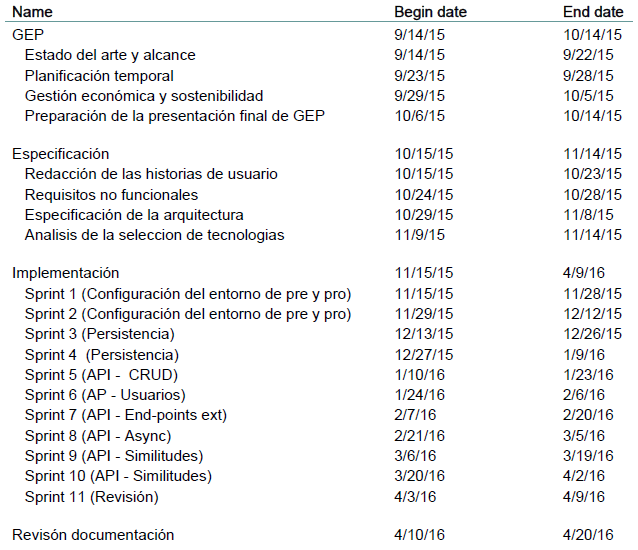
\includegraphics[width=\textwidth,height=\textheight,keepaspectratio]{add/Task.png}
\label{fig:task}
\end{figure}

\newpage
\subsubsection{Gráfico gantt}

\begin{figure}[ht!]
\center
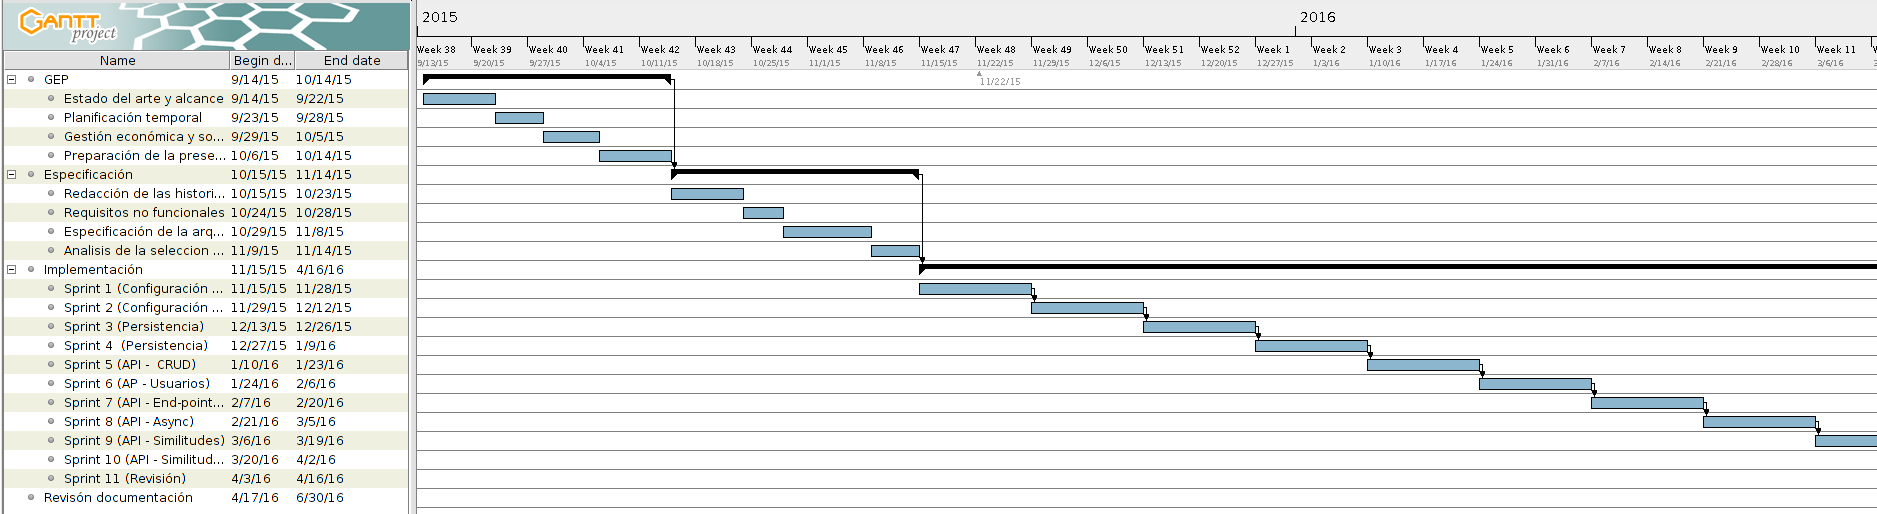
\includegraphics[width=\textwidth,height=\textheight,keepaspectratio]{add/Gantt_1.png}
\label{fig:gantt_1}
\end{figure}


\begin{figure}[ht!]
\center
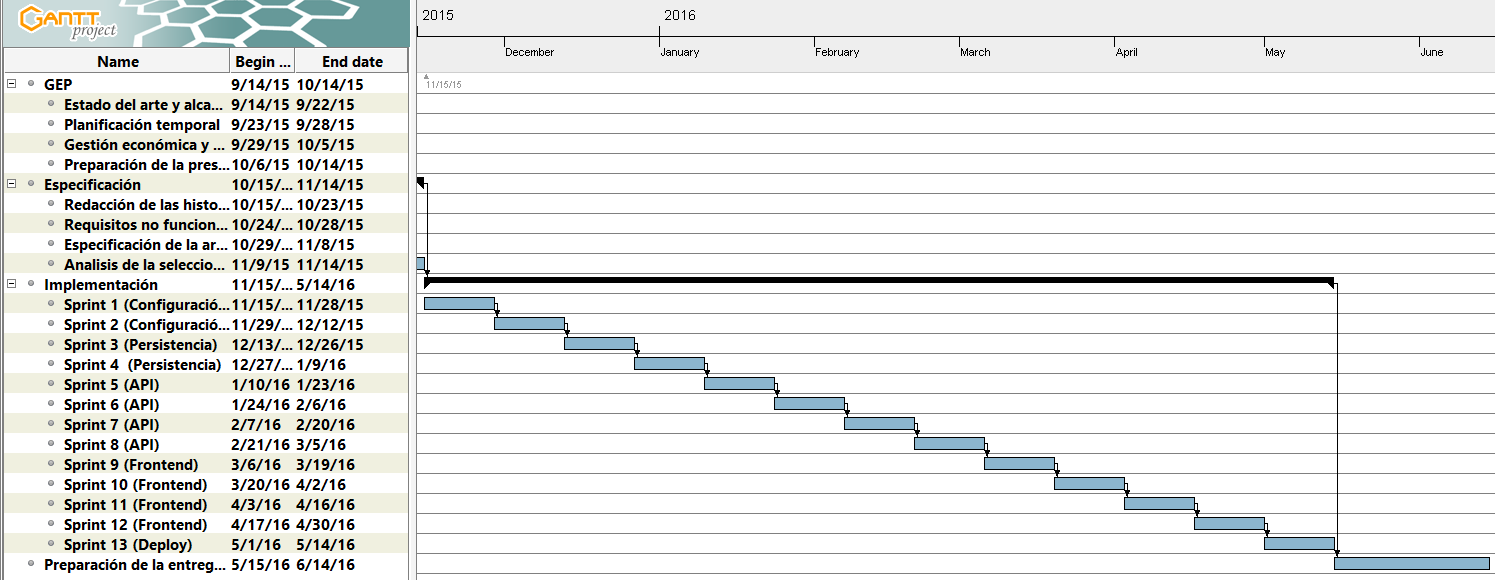
\includegraphics[width=\textwidth,height=\textheight,keepaspectratio]{add/Gantt_2.png}
\label{fig:gantt_2}
\end{figure}

\end{landscape}
\newpage

\subsection{Recursos}
Las necesidades en recursos serán muy escuetas dado que todo el software que se usara es libre y las maquinas en las que se trabaja en preprducción serán virtuales. La única necesidad de tener unos recursos que se necesiten planificar, ya que requieren ser contratados, son los servidores en los que se hará el \textit{deploy}, se tendrán que contratar durante las semanas que dures los \textit{sprints} en los que se haga el \textit{deploy.}

\subsection{Alterativas y plan de acción}
Dado que el proyecto se desarrollara usando \textit{Scrum}, al final de cada \textit{sprint}, durante el \textit{sprint backlog} se determinara si se han  
cumplido las expectativas del \textit{sprint}. Por otro lado en el \textit{sprint planning} se tendrá en cuenta si han habido carencias o bugs en los anteriores \textit{sprints} para incorporarlos como historias de usuario al siguiente \textit{sprint}. 

Como se ha comentado en el alcance, se diseñara un software abierto orientado al desarrollo continuado. Por lo que en el sprint 13 se dará por concluido el proyecto, y se documentara el estado en el que se encuentre y las historias de usuario pendientes.

\end{document}



